\chapter{Ottimizzazione mediante Istruzioni SIMD}
\label{cap:simd}

\section{Dove Intervenire}

Quasi tutto il tempo di esecuzione è speso nella prima fase, e al suo interno nel calcolo delle distanze: nelle misure del Capitolo~\ref{cap:sperimentazione} la costruzione del Ball Tree e l'espansione dei cluster pesano insieme meno del 2\% del totale. Il candidato naturale per le istruzioni SIMD (\emph{Single Instruction, Multiple Data}) è quindi il calcolo della distanza al quadrato tra due punti, che applica la stessa sequenza di operazioni --- sottrazione, quadrato, somma --- a tutte le coordinate. Il secondo kernel, il riempimento del vettore delle etichette con un valore costante, è eseguito una sola volta per esecuzione e ha un peso trascurabile; è mantenuto perché era parte dell'esercizio del corso e mostra le istruzioni su dati interi.

Entrambi i kernel sono scritti in assembly NASM, uno per architettura, e dichiarati in \codice{kernels.h} con puntatori e dimensioni come parametri:

\begin{lstlisting}[language=C]
real_t dist2_simd(const real_t *a, const real_t *b, int d);
void fill_labels_simd(int *labels, int n, int value);
\end{lstlisting}

Nella versione d'esame le funzioni assembly ricevevano invece il puntatore alla struttura dei parametri e ne leggevano i campi a spiazzamenti fissi, per esempio \codice{[rdi+40]} per la dimensione: una modifica alla struttura bastava a rompere il codice assembly senza alcun errore di compilazione. Con i puntatori, inoltre, lo stesso kernel serve sia per la distanza tra due righe del dataset sia per quella tra un punto e il centro di una sfera del Ball Tree.

\section{Il Kernel a 32 Bit con SSE}

Nella variante a 32 bit i valori sono \codice{float} e un registro XMM ne contiene quattro. Il Listato~\ref{lst:kernel32} riporta il kernel della distanza.

\begin{lstlisting}[language=nasm, caption={Distanza al quadrato con SSE (\codice{src/asm/kernels32.nasm}).}, label={lst:kernel32}]
dist2_simd:
        mov     eax, [esp+4]            ; a
        mov     ecx, [esp+8]            ; b
        mov     edx, [esp+12]           ; d
        shl     edx, 2                  ; lunghezza della riga in byte
        add     eax, edx                ; puntatori alla fine delle righe,
        add     ecx, edx                ; percorse con uno spiazzamento negativo
        neg     edx
        xorps   xmm0, xmm0              ; 4 somme parziali
.loop:
        movaps  xmm1, [eax+edx]         ; 4 coordinate di a
        subps   xmm1, [ecx+edx]         ; meno 4 coordinate di b
        mulps   xmm1, xmm1
        addps   xmm0, xmm1
        add     edx, 16
        jnz     .loop
        haddps  xmm0, xmm0              ; somma orizzontale (SSE3)
        haddps  xmm0, xmm0
        sub     esp, 4                  ; st(0) si carica solo dalla memoria
        movss   [esp], xmm0
        fld     dword [esp]
        add     esp, 4
        ret
\end{lstlisting}

Alcune scelte meritano un commento:

\begin{itemize}
    \item \textbf{Ciclo a spiazzamento negativo.} I puntatori sono spostati alla fine delle righe e il ciclo le percorre con un indice negativo che cresce fino a zero: l'istruzione \codice{add} che aggiorna l'indice imposta anche il flag di zero, e il ciclo non ha bisogno di un confronto separato.
    \item \textbf{Nessun residuo.} Grazie al padding (Sezione~\ref{sec:padding}) la dimensione è sempre un multiplo di quattro e le righe sono allineate, quindi il ciclo lavora solo su blocchi interi con caricamenti allineati.
    \item \textbf{Somme parziali.} L'accumulatore contiene quattro somme parziali indipendenti, ridotte a una sola alla fine con due \codice{haddps}.
    \item \textbf{Valore di ritorno.} La convenzione di chiamata \emph{cdecl} a 32 bit~\cite{sysv} prevede che una funzione restituisca i valori in virgola mobile in cima allo stack del coprocessore x87, \codice{st(0)}. Non è quindi una scelta, come riportava la relazione d'esame, ma un obbligo. Poiché \codice{st(0)} si può caricare solo dalla memoria, il valore passa per una cella sullo stack del thread. La versione d'esame usava invece una variabile globale: due thread che eseguono il kernel contemporaneamente scrivono nella stessa cella, e uno dei due può restituire la distanza calcolata dall'altro.
    \item \textbf{Registri.} La convenzione impone di preservare \codice{EBX}, \codice{ESI}, \codice{EDI} e \codice{EBP}; il kernel usa solo \codice{EAX}, \codice{ECX}, \codice{EDX} e registri XMM, che il chiamante non si aspetta di ritrovare intatti, e quindi non deve salvare nulla.
\end{itemize}

\section{Il Kernel a 64 Bit con AVX}

Nella variante a 64 bit i valori sono \codice{double} e i registri YMM a 256 bit dell'estensione AVX ne contengono quattro, così che la struttura del ciclo resta la stessa (Listato~\ref{lst:kernel64}). La convenzione di chiamata è quella System V AMD64~\cite{sysv}: i primi argomenti interi arrivano in \codice{RDI}, \codice{RSI} e \codice{RDX}, il risultato in virgola mobile si restituisce in \codice{XMM0}.

\begin{lstlisting}[language=nasm, caption={Distanza al quadrato con AVX (\codice{src/asm/kernels64.nasm}).}, label={lst:kernel64}]
dist2_simd:
        movsxd  rdx, edx
        shl     rdx, 3                  ; lunghezza della riga in byte
        add     rdi, rdx
        add     rsi, rdx
        neg     rdx
        vxorpd  ymm0, ymm0, ymm0        ; 4 somme parziali
.loop:
        vmovapd ymm1, [rdi+rdx]
        vsubpd  ymm1, ymm1, [rsi+rdx]
        vmulpd  ymm1, ymm1, ymm1
        vaddpd  ymm0, ymm0, ymm1
        add     rdx, 32
        jnz     .loop
        vextractf128 xmm1, ymm0, 1      ; somma la meta' alta alla bassa
        vaddpd  xmm0, xmm0, xmm1
        vhaddpd xmm0, xmm0, xmm0        ; e le due corsie rimaste
        vzeroupper
        ret
\end{lstlisting}

\begin{figure}[H]
    \centering
    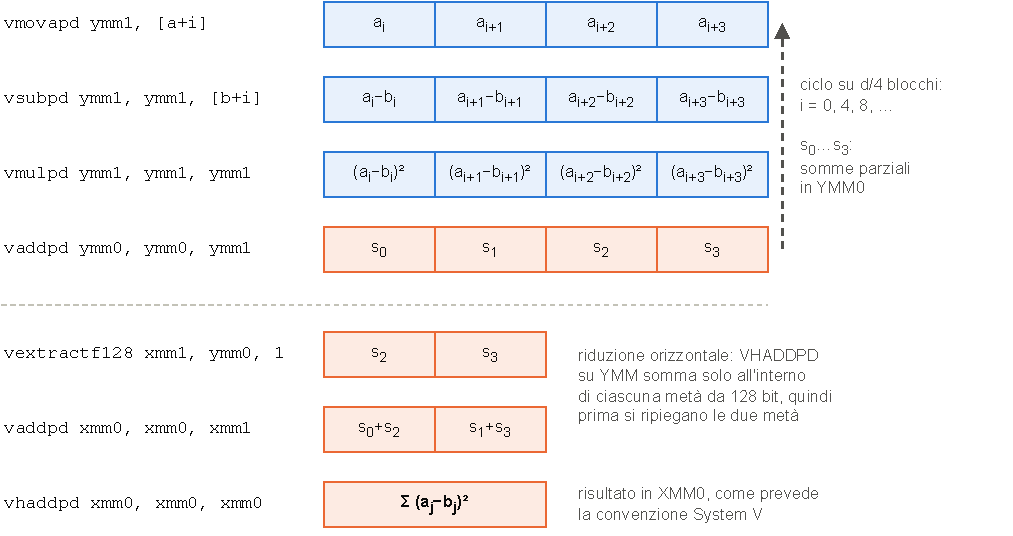
\includegraphics[width=\textwidth]{diagrammi/simd.pdf}
    \caption{Una iterazione del kernel AVX e la riduzione finale delle quattro somme parziali.}
    \label{fig:simd}
\end{figure}

La riduzione finale (Figura~\ref{fig:simd}) è diversa da quella a 32 bit perché \codice{vhaddpd} su registri YMM somma le coppie di valori all'interno di ciascuna metà da 128 bit, senza mai combinare le due metà: occorre prima estrarre la metà alta con \codice{vextractf128} e sommarla a quella bassa. Prima di tornare al chiamante, \codice{vzeroupper} azzera la metà alta dei registri YMM. Sui processori Intel~\cite{intel}, eseguire istruzioni SSE non codificate VEX mentre le metà alte sono \enquote{sporche} comporta una penalità di transizione, e il codice C compilato da GCC nel chiamante può contenerne. Per lo stesso motivo il kernel usa solo istruzioni con codifica VEX, mentre il kernel d'esame alternava istruzioni AVX e SSE (\codice{movsd}, \codice{subsd}, \codice{sqrtsd}) nello stesso ciclo e non eseguiva \codice{vzeroupper}.

Anche qui il kernel usa solo registri che la convenzione non chiede di preservare. Il kernel d'esame salvava invece quattro registri con \codice{push rax, rbx, rcx, rdi} e li ripristinava con \codice{pop} nello stesso ordine, anziché in ordine inverso: al ritorno \codice{RBX}, che il chiamante si aspetta invariato, conteneva il valore di \codice{RCX}. Il programma funzionava solo perché il codice generato con \codice{-O0} non usava \codice{RBX} in quel punto. Nella stessa versione, la macro \codice{popaq} fornita con il template ripristinava anche i registri YMM, sovrascrivendo il risultato appena calcolato in \codice{XMM0}: è questo il comportamento osservato nella relazione d'esame e attribuito, erroneamente, al processore.

\section{Il Riempimento delle Etichette}

\codice{fill\_labels\_simd} replica un intero in tutte le corsie di un registro e lo scrive a blocchi: quattro etichette per istruzione con SSE (\codice{pshufd} e \codice{movdqa}), otto con AVX. L'estensione AVX non dispone di rimescolamenti su interi a 256 bit, quindi il valore viene replicato in un registro XMM e copiato nella metà alta con \codice{vinsertf128}. Un breve ciclo scalare scrive le etichette residue quando $n$ non è multiplo della larghezza del registro. Rispetto alla versione d'esame, il valore da scrivere è un parametro invece di una costante in memoria, e le condizioni di uscita sono corrette per ogni $n$, compresi i valori minori di quattro.

\section{Confronto con il Codice del Compilatore}
\label{sec:compilatore}

Il template del corso prescriveva la compilazione con \codice{-O0}, per rendere evidente il contributo del codice assembly. La versione attuale è compilata con \codice{-O2}, e a questo livello GCC vettorizza da sé il ciclo della versione C del kernel. Il codice generato (Listato~\ref{lst:gcc}) mostra però che la vettorizzazione è solo parziale.

\begin{lstlisting}[language=nasm, caption={Ciclo di \codice{dist2\_c} generato da GCC 16 con \codice{-O2 -mavx} (sintassi AT\&T).}, label={lst:gcc}]
.L4:    vmovupd     (%rdi,%rax), %ymm1
        vsubpd      (%rsi,%rax), %ymm1, %ymm1
        addq        $32, %rax
        vmulpd      %ymm1, %ymm1, %ymm1
        vaddsd      %xmm1, %xmm0, %xmm0
        vunpckhpd   %xmm1, %xmm1, %xmm2
        vextractf128 $0x1, %ymm1, %xmm1
        vaddsd      %xmm2, %xmm0, %xmm0
        vaddsd      %xmm1, %xmm0, %xmm0
        vunpckhpd   %xmm1, %xmm1, %xmm1
        vaddsd      %xmm1, %xmm0, %xmm0
        cmpq        %rcx, %rax
        jne         .L4
\end{lstlisting}

Sottrazioni e quadrati sono calcolati quattro alla volta, ma i quadrati vengono poi sommati all'accumulatore uno per volta, in ordine, con quattro \codice{vaddsd} dipendenti l'una dall'altra. La somma in virgola mobile non è associativa, e senza un permesso esplicito (\codice{-ffast-math} o \codice{-fassociative-math}) il compilatore non può cambiare l'ordine delle addizioni. Il kernel scritto a mano lo cambia deliberatamente, mantenendo quattro somme parziali indipendenti, e completa un'iterazione con una sola somma vettoriale invece di una catena di quattro. Il risultato può differire da quello sequenziale nelle ultime cifre, ma i test del Capitolo~\ref{cap:sperimentazione} verificano che le etichette non cambiano. La Sezione~\ref{sec:esp-compilatore} misura il vantaggio che resta al codice scritto a mano con entrambi i livelli di ottimizzazione.
